\chapter{Model personalisation}
\label{chp:personalisation}
Introduction to chapter

Recap findings and shortcomings from the previous chapter
What classification performance are we trying to beat? Look back at previous chapter to find performance target

What are the aims of this chapter?
- Develop methods to produce models that perform better for an individual 
- Identify requirements for implementing these methods (data, computation)
- Demonstrate performance improvements and limitations of the methods
Relate these issues to the research questions for the thesis in general

Research question?
Focusing on the data of an individual how performant a model can be achieved
Can a large population of data be effectively used to improve the performance of this individual trained model. "Given a small amount of labelled target data, how should we combine it during training with the large amount of labelled source data to achieve the lowest target error at test time?"



Transfer learning approaches focus on reducing the labelling requirements for training data.

%------------------------------------------
% \section{Theory}
% Theory introduction - what is important for this section
% - How do ML models learn]
% - Transfer learning/Domain adaptation

%------------------------------------------
\section{Related Works} % TODO: THIS SHOULD BE SPLIT INTO THEORY AND RELATED WORKS
% Introduction
"The ultimate goal of transfer learning is to reduce labeled data requirements by exploiting a pre-existing embedding model trained for different datasets or tasks" \cite{Shor2020}

"In contrast to the traditional machine learning and data mining techniques, which assume that the training and testing data lie from the same feature space and distribution, transfer learning can handle situations where there is a discrepancy between domains and distributions. These characteristics give the model the potential to utilize the available related source data and extend the underlying knowledge to the target task achieving better performance"\cite{Farahani2020}

% Some generic descriptions of related works in this field x and y did this. This is a common theme etc
deep transfer learning - knowledge transfer between different data sets with sensors in different places\cite{Wang2018a}

Two common schemes are employed in literature to achieve personalisation from source to target - retraining of a general model, tuning of a domain mapping function

% Domain adaptation - Create mapping between similar subjects
Joint probability domain adaptation and improved pseudo labels\cite{Fu2021}. Manually selected features. Domain adaptation through selection of a mapping function between source and target features. 93.3\% accuracy of target domain

% Retrain general model
Personalised language modelling using RNN - no examples of transfer learning for HAR in RNN. "It trains a base model with a large dataset and copies its first n-many layers to the first n-many layers of a target model. Then the target model is fine-tuned with relatively small target data. Several learning schemes such as freezing a certain layer or adding a surplus layer are pro- posed for achieving the result."\cite{Yoon2017}

% Training from similar users
Similarity based personalisation strategies. Comparison of physical characteristics of different subjects\cite{Ferrari2020}. Adaboost classifier. Train using data from a general population, with and without some of the target subject's data. Similarity between different subjects is used to weight the influence of a subjects data.

% Combination - retrain general model based on similar users
Cruciani et al presents work on personalising an activity recognition model built from the subset of a general population. The subset of subjects was selected by comparing the similarity of manually selected features for the target subject and general training population. Those with the closest matching gait are used to generate the base model. Further training is then performed on this model using a small amount of the target subject data. This approach achieved a ~5\% improvement in performance when compared to selecting a subset at random\cite{Cruciani2020}. The experiment was performed on the \acrshort{adl} Extrasensory dataset published by Vaizman et al\cite{Vaizman2017}.

Research gaps
- Transfer learning in HAR has only used manually selected features - not learnt (deep) features
- Limited exploration of transfer learning for RNN in HAR

%------------------------------------------
\section{Methods and Materials}
Extended the data set previously captured for a select subset of participants. The same methods as presented in Section \ref{sec:methods-data-collection} were used to collect this additional data.

Larger quantities of data collected for 3 subjects least 7-mins cumulative time of each activity class. 

To perform machine learning on just a single participant a different data division method is required than in the previous work. Instead using participants as the division point. Transitions between activity was used as previously described in \ref{par:methods-per-episode-division}.

What kind of ML model are we going to use?
% TODO: Add in LSTM model being tested
\begin{figure}[htbp]
    \centering
    \includegraphics[width=0.6\textwidth]{example-image-duck}
    \caption{Illustration of LSTM model that is being tested}
    \label{fig:ch5_illustration_of_base_LSTM_model}
\end{figure}


How are we going to perform our personalisation/transfer learning
% Train with a mixture of both target and source data
% Re-train a pre-trained model
% Freezing trainable parameters on set layers to 


How are we going to determine performance? Categorical accuracy, Confusion Matrices, F1-Scores
% What would better than the baseline look like. Less data, faster at training, better performance

\begin{figure}[htbp]
    \centering
    \includegraphics[width=0.6\textwidth]{example-image-duck}
    \caption{LSTM Setups for transfer learning}
    \label{fig:ch5_LSTM_model_transfer_learning}
\end{figure}



\section{Results and Analysis}
The following sections contains the results and analysis of personalisation experiments. This split up into two sections, the first, Section \ref{subsec:ch5-baseline-model-results} looks at determining a baseline for personalisation performance. The second, Section \ref{subsec:ch5-model-personalisation-results} looks at new methods for improving this performance using data from additional individuals.

\subsection{Baseline Model}
\label{subsec:ch5-baseline-model-results}
Want to determine a baseline performance that can be achieved using only one individuals data. If performance of new methods does not exceed this value there is no benefit in the methods. Feed in increasing amounts of training data into the training process and see what performance improvements can be seen.

% Training performance vs quantity of data for both subjects
X axis is windows of data per class. Each window is 128 samples long at 100Hz, with a skip value of 3 samples so from 30 seconds per class to 450 seconds per class. Test samples was fixed at 5000 samples for all evaluations - 151 seconds

Figure \ref{fig:ch5_bespoke_mode_classification} shows the classification performance for the three Target subjects for different amounts of target data windows and different sized LSTM networks. Full data tables are available in Appendix \ref{sec:appendix-a-model-performance-bespoke}.

\begin{figure}[p]
    \centering
    \begin{subfigure}[b]{0.9\textwidth}
        \centering
        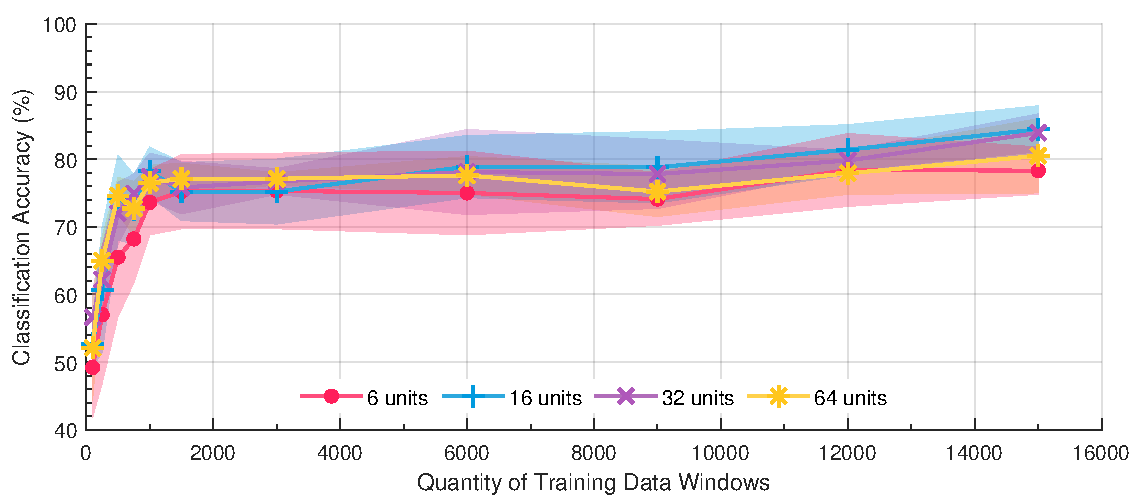
\includegraphics[width=\textwidth]{content/5-Personalisation/Bespoke_Target/ch5_bespoke_target_model_subject_1.pdf}
        \caption{Subject 01}
        \label{fig:ch5_6_unit_bespoke_model}
    \end{subfigure}
    \begin{subfigure}[b]{0.9\textwidth}
        \centering
        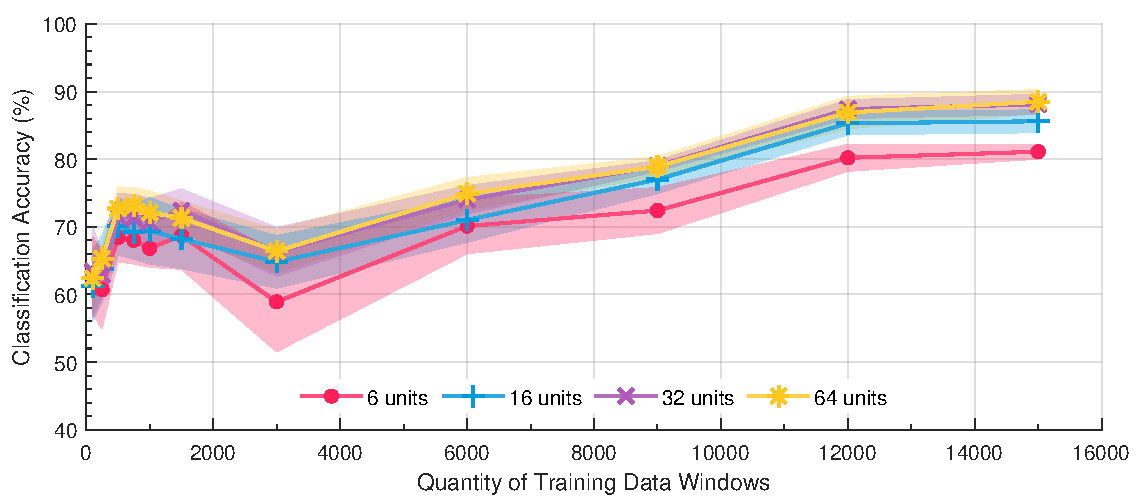
\includegraphics[width=\textwidth]{content/5-Personalisation/Bespoke_Target/ch5_bespoke_target_model_subject_3.pdf}
        \caption{Subject 03}
        \label{fig:ch5_16_unit_bespoke_model}
    \end{subfigure}
    \begin{subfigure}[b]{0.9\textwidth}
        \centering
        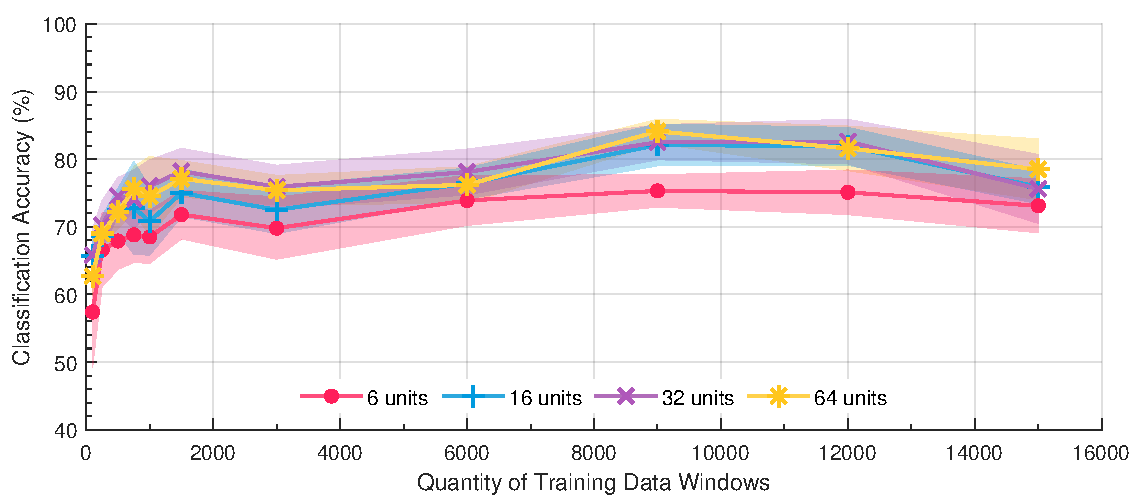
\includegraphics[width=\textwidth]{content/5-Personalisation/Bespoke_Target/ch5_bespoke_target_model_subject_9.pdf}
        \caption{Subject 09}
        \label{fig:ch5_32_unit_bespoke_model}
    \end{subfigure}
    \caption[TODO Caption]{\hl{TODO Caption}}
    \label{fig:ch5_bespoke_mode_classification}
\end{figure}

Maximum performance achieved was 84.4\% for Subject 01, 88.5\% for Subject 03, and 82.6\% for Subject 09.

Performance improves rapidly from 100 to 1500 data samples, there is then a gradual increase in performance for the remaining increases in training windows.

Performance appears to still be increasing when the maximum amount of data was tested. Indicating further data would still improve performance. Not realistic to expose the model to every possible environment that it will need to operate on.

Standard deviation reduces with increasing data windows indicating more consistent performance across the 5 test sets.

Reduction in performance at 3000 samples for Subject 03 is likely due to model exposure to a new environment of data. Performance recovers with increasing amounts of data. Subject 09 also experiences similar drops in performance.

Increasing the number of units in general improved classification performance. This levels off at 32 units. Increasing the number of units also reduced the number of epochs required to train the models.

%Why is the model not achieving better performance?
By looking at the confusion matrices it can be seen which classes the models are struggling to identify. Table \ref{tab:ch5-bespoke-mode-confusion-matrix_subject_09} shows confusion matrices for the three targets subjects when the model is presented with test data.

\begin{table}[htbp]
    \centering
    \caption[Confusion matrix of test data for a 32 unit trained with \hl{x} target data LSTM model]{\hl{TODO: Put in correct values}Confusion matrix of test data for a 32 unit trained with \hl{x} target data LSTM model. (\acrfull{ra}, \acrfull{rd}, \acrfull{sa}, \acrfull{sd})}
    \label{tab:ch5-bespoke-mode-confusion-matrix_subject_09}
    \begin{subtable}{\textwidth}
    \caption{Subject 01}
    \begin{tabularx}{\textwidth}{ccYYYYYY}
        \noalign{\hrule height 1.5pt}
         & & \multicolumn{6}{c}{\textbf{Predicted Classes}} \\
         \hline
         & & WALK & \acrshort{ra} & \acrshort{rd} & \acrshort{sa} & \acrshort{sd} & STOP \\
         \multirow{6}{*}{\rotatebox{90}{\textbf{True Classes}}} 
         & WALK          & 100\% & 0 & 0 & 0 & 0 & 0 \\
         & \acrshort{ra} & 0 & 98\% & 2\% & 0 & 0 & 0 \\
         & \acrshort{rd} & 0 & 0 & 100\% & 0 & 0 & 0 \\
         & \acrshort{sa} & 0 & 0 & 0 & 100\% & 0 & 0 \\
         & \acrshort{sd} & 0 & 0 & 0 & 0 & 100\% & 0 \\
         & STOP          & 0 & 0 & 0 & 0 & 0 & 100\% \\
         \noalign{\hrule height 1.5pt}
    \end{tabularx}
    \end{subtable}
    \ \\ \vspace{0.3cm}
    \begin{subtable}{\textwidth}
    \caption{Subject 03}
    \begin{tabularx}{\textwidth}{ccYYYYYY}
        \noalign{\hrule height 1.5pt}
         & & \multicolumn{6}{c}{\textbf{Predicted Classes}} \\
         \hline
         & & WALK & \acrshort{ra} & \acrshort{rd} & \acrshort{sa} & \acrshort{sd} & STOP \\
         \multirow{6}{*}{\rotatebox{90}{\textbf{True Classes}}} 
         & WALK          & 100\% & 0 & 0 & 0 & 0 & 0 \\
         & \acrshort{ra} & 0 & 98\% & 2\% & 0 & 0 & 0 \\
         & \acrshort{rd} & 0 & 0 & 100\% & 0 & 0 & 0 \\
         & \acrshort{sa} & 0 & 0 & 0 & 100\% & 0 & 0 \\
         & \acrshort{sd} & 0 & 0 & 0 & 0 & 100\% & 0 \\
         & STOP          & 0 & 0 & 0 & 0 & 0 & 100\% \\
         \noalign{\hrule height 1.5pt}
    \end{tabularx}
    \end{subtable}
    \ \\ \vspace{0.3cm}
    \begin{subtable}{\textwidth}
    \caption{Subject 09}
    \begin{tabularx}{\textwidth}{ccYYYYYY}
        \noalign{\hrule height 1.5pt}
         & & \multicolumn{6}{c}{\textbf{Predicted Classes}} \\
         \hline
         & & WALK & \acrshort{ra} & \acrshort{rd} & \acrshort{sa} & \acrshort{sd} & STOP \\
         \multirow{6}{*}{\rotatebox{90}{\textbf{True Classes}}} 
         & WALK          & 100\% & 0 & 0 & 0 & 0 & 0 \\
         & \acrshort{ra} & 0 & 98\% & 2\% & 0 & 0 & 0 \\
         & \acrshort{rd} & 0 & 0 & 100\% & 0 & 0 & 0 \\
         & \acrshort{sa} & 0 & 0 & 0 & 100\% & 0 & 0 \\
         & \acrshort{sd} & 0 & 0 & 0 & 0 & 100\% & 0 \\
         & STOP          & 0 & 0 & 0 & 0 & 0 & 100\% \\
         \noalign{\hrule height 1.5pt}
    \end{tabularx}
    \end{subtable}
\end{table}

Talk about f-scores - indicate poor performance for Walking, Ramp Ascent and Ramp Descent
% Present graph of Learning rate

% Analysis points points
% - Why did subject x perform worse
% - Would more data help?
% - What baseline does this set for our subsequent work

\subsection{Model Personalisation}
\label{subsec:ch5-model-personalisation-results}
% Introductory paragraph

% Aims of this experiment - determine if using additional data from other individuals can improve the performance of a bespoke model

% \subsection{Results and Analysis}
% % Introductory Paragraph

\subsubsection{Mixing Target and Source Data}
% Fully trained model
% Present performance on this model - Categorical accuracy of training data, learning rate (epochs vs categorical accuracy)
\begin{landscape}
% Subject 01 - classification accuracy for varying source and target data
\begin{table}[p]
    \centering
    \caption[Table of classification accuracy for Subject 01 for a model trained using varying amounts of Source and Target training data]{Table of classification accuracy for Subject 01 for a model trained using varying amounts of Source and Target training data. The cell value represents the percentage classification accuracy $\pm\sigma$. The highest classification accuracy has been highlighted in bold.}
    \ \\
    \label{tab:ch5-mixed-target-and-source-data-subject-01}
    \begin{tabular}{cr| *{7}{C{2cm}}}
        \noalign{\hrule height 1.5pt}
         & & \multicolumn{7}{c}{\textbf{Source Training Windows}}\\
         & & 100 & 250 & 500 & 750 & 1000 & 1500 & 3000 \\
         \hline
         
         \multirow{11}{*}{\rotatebox{90}{\parbox{5.3cm}{\centering\textbf{Target Training Windows}}}}
         
         & 100 & $0.601{\scriptscriptstyle\pm0.07}$ & $0.630{\scriptscriptstyle\pm0.06}$ & $0.587{\scriptscriptstyle\pm0.05}$ & $0.620{\scriptscriptstyle\pm0.02}$ & $0.572{\scriptscriptstyle\pm0.06}$ & $0.587{\scriptscriptstyle\pm0.04}$ & $0.592{\scriptscriptstyle\pm0.04}$ \\
         & 250 & $0.609{\scriptscriptstyle\pm0.08}$ & $0.696{\scriptscriptstyle\pm0.04}$ & $0.643{\scriptscriptstyle\pm0.05}$ & $0.649{\scriptscriptstyle\pm0.06}$ & $0.631{\scriptscriptstyle\pm0.06}$ & $0.630{\scriptscriptstyle\pm0.08}$ & $0.651{\scriptscriptstyle\pm0.02}$ \\
         & 500   & $0.743{\scriptscriptstyle\pm0.02}$ & $0.713{\scriptscriptstyle\pm0.04}$ & $0.741{\scriptscriptstyle\pm0.02}$ & $0.731{\scriptscriptstyle\pm0.04}$ & $0.711{\scriptscriptstyle\pm0.04}$ & $0.727{\scriptscriptstyle\pm0.03}$ & $0.737{\scriptscriptstyle\pm0.04}$ \\
         & 750  & $0.736{\scriptscriptstyle\pm0.03}$ & $0.708{\scriptscriptstyle\pm0.06}$ & $0.721{\scriptscriptstyle\pm0.03}$ & $0.747{\scriptscriptstyle\pm0.02}$ & $0.731{\scriptscriptstyle\pm0.03}$ & $0.735{\scriptscriptstyle\pm0.04}$ & $0.782{\scriptscriptstyle\pm0.03}$ \\
         & 1000 & $0.769{\scriptscriptstyle\pm0.02}$ & $0.782{\scriptscriptstyle\pm0.04}$ & $0.748{\scriptscriptstyle\pm0.01}$ & $0.768{\scriptscriptstyle\pm0.02}$ & $0.768{\scriptscriptstyle\pm0.05}$ & $0.775{\scriptscriptstyle\pm0.03}$ & $0.772{\scriptscriptstyle\pm0.02}$ \\
         & 1500  & $0.769{\scriptscriptstyle\pm0.05}$ & $0.778{\scriptscriptstyle\pm0.02}$ & $0.781{\scriptscriptstyle\pm0.04}$ & $0.758{\scriptscriptstyle\pm0.02}$ & $0.757{\scriptscriptstyle\pm0.01}$ & $0.793{\scriptscriptstyle\pm0.05}$ & $0.770{\scriptscriptstyle\pm0.04}$ \\
         & 3000  & $0.774{\scriptscriptstyle\pm0.04}$ & $0.756{\scriptscriptstyle\pm0.05}$ & $0.787{\scriptscriptstyle\pm0.02}$ & $0.730{\scriptscriptstyle\pm0.03}$ & $0.741{\scriptscriptstyle\pm0.02}$ & $0.786{\scriptscriptstyle\pm0.02}$ & $0.776{\scriptscriptstyle\pm0.02}$ \\
         & 6000  & $0.799{\scriptscriptstyle\pm0.06}$ & $0.797{\scriptscriptstyle\pm0.03}$ & $0.764{\scriptscriptstyle\pm0.06}$ & $0.773{\scriptscriptstyle\pm0.04}$ & $0.754{\scriptscriptstyle\pm0.03}$ & $0.774{\scriptscriptstyle\pm0.02}$ & $0.792{\scriptscriptstyle\pm0.05}$ \\
         & 9000  & $0.749{\scriptscriptstyle\pm0.04}$ & $0.781{\scriptscriptstyle\pm0.05}$ & $0.785{\scriptscriptstyle\pm0.04}$ & $0.767{\scriptscriptstyle\pm0.06}$ & $0.743{\scriptscriptstyle\pm0.03}$ & $0.754{\scriptscriptstyle\pm0.03}$ & $0.752{\scriptscriptstyle\pm0.04}$ \\
         & 12000 & $0.805{\scriptscriptstyle\pm0.03}$ & $0.754{\scriptscriptstyle\pm0.07}$ & $0.798{\scriptscriptstyle\pm0.04}$ & $0.782{\scriptscriptstyle\pm0.05}$ & $0.816{\scriptscriptstyle\pm0.02}$ & $0.777{\scriptscriptstyle\pm0.04}$ & $0.794{\scriptscriptstyle\pm0.02}$ \\
         & 15000 & $0.855{\scriptscriptstyle\pm0.03}$ & $0.822{\scriptscriptstyle\pm0.04}$ & $0.848{\scriptscriptstyle\pm0.02}$ & $\mathbf{0.861{\scriptscriptstyle\pm0.02}}$ & $0.836{\scriptscriptstyle\pm0.05}$ & $0.829{\scriptscriptstyle\pm0.02}$ & $0.833{\scriptscriptstyle\pm0.02}$ \\
         \noalign{\hrule height 1.5pt}
    \end{tabular}
    \ \\ \vspace{0.5cm}
    \begin{tabular}{cr| *{4}{C{2cm}}}
        \noalign{\hrule height 1.5pt}
         & & \multicolumn{4}{c}{\textbf{Source Training Windows}}\\
         & & 6000 & 9000 & 12000 & 15000 \\
         \hline
         \multirow{11}{*}{\rotatebox{90}{\parbox{5.3cm}{\centering\textbf{Target Training Windows}}}}
         
         & 100 & $0.590{\scriptscriptstyle\pm0.07}$ & $0.584{\scriptscriptstyle\pm0.03}$ & $0.618{\scriptscriptstyle\pm0.03}$ & $0.593{\scriptscriptstyle\pm0.02}$ \\
         
        & 250 & $0.670{\scriptscriptstyle\pm0.02}$ & $0.617{\scriptscriptstyle\pm0.04}$ & $0.661{\scriptscriptstyle\pm0.05}$ & $0.685{\scriptscriptstyle\pm0.04}$ \\
        
        & 500 & $0.713{\scriptscriptstyle\pm0.06}$ & $0.731{\scriptscriptstyle\pm0.02}$ & $0.754{\scriptscriptstyle\pm0.03}$ & $0.716{\scriptscriptstyle\pm0.05}$ \\
        
        & 750 & $0.746{\scriptscriptstyle\pm0.02}$ & $0.729{\scriptscriptstyle\pm0.03}$ & $0.782{\scriptscriptstyle\pm0.03}$ & $0.743{\scriptscriptstyle\pm0.03}$ \\
        
        & 1000 & $0.774{\scriptscriptstyle\pm0.04}$ & $0.748{\scriptscriptstyle\pm0.02}$ & $0.761{\scriptscriptstyle\pm0.03}$ & $0.771{\scriptscriptstyle\pm0.01}$ \\
        
        & 1500 & $0.789{\scriptscriptstyle\pm0.04}$ & $0.786{\scriptscriptstyle\pm0.05}$ & $0.746{\scriptscriptstyle\pm0.04}$ & $0.731{\scriptscriptstyle\pm0.02}$ \\
        
        & 3000 & $0.770{\scriptscriptstyle\pm0.01}$ & $0.764{\scriptscriptstyle\pm0.02}$ & $0.776{\scriptscriptstyle\pm0.01}$ & $0.755{\scriptscriptstyle\pm0.05}$ \\ 
        
        & 6000 & $0.794{\scriptscriptstyle\pm0.01}$ & $0.805{\scriptscriptstyle\pm0.03}$ & $0.763{\scriptscriptstyle\pm0.06}$ & $0.775{\scriptscriptstyle\pm0.03}$ \\
        
        & 9000 & $0.765{\scriptscriptstyle\pm0.04}$ & $0.751{\scriptscriptstyle\pm0.04}$ & $0.776{\scriptscriptstyle\pm0.06}$ & $0.761{\scriptscriptstyle\pm0.03}$ \\
        
        & 12000 & $0.789{\scriptscriptstyle\pm0.04}$ & $0.813{\scriptscriptstyle\pm0.04}$ & $0.773{\scriptscriptstyle\pm0.02}$ & $0.801{\scriptscriptstyle\pm0.01}$ \\
        
        & 15000 & $0.846{\scriptscriptstyle\pm0.04}$ & $0.846{\scriptscriptstyle\pm0.01}$ & $0.843{\scriptscriptstyle\pm0.02}$ & $0.852{\scriptscriptstyle\pm0.01}$ \\
        
        \noalign{\hrule height 1.5pt}
    \end{tabular}
\end{table}

% Subject 03 - classification accuracy for varying source and target data
\begin{table}[p]
    \centering
    \caption[Table of classification accuracy for Subject 03 for a model trained using varying amounts of Source and Target training data]{Table of classification accuracy for Subject 03 for a model trained using varying amounts of Source and Target training data. The cell value represents the percentage classification accuracy $\pm\sigma$. The highest classification accuracy has been highlighted in bold.}
    \ \\
    \label{tab:ch5-mixed-target-and-source-data-subject-03}
    \begin{tabular}{cr| *{7}{C{2cm}}}
        \noalign{\hrule height 1.5pt}
         & & \multicolumn{7}{c}{\textbf{Source Training Windows}}\\
         & & 100 & 250 & 500 & 750 & 1000 & 1500 & 3000 \\
         \hline
         
         \multirow{11}{*}{\rotatebox{90}{\parbox{5.3cm}{\centering\textbf{Target Training Windows}}}}
         
        & 100 & $0.635{\scriptscriptstyle\pm0.05}$ & $0.682{\scriptscriptstyle\pm0.01}$ & $0.662{\scriptscriptstyle\pm0.02}$ & $0.670{\scriptscriptstyle\pm0.05}$ & $0.658{\scriptscriptstyle\pm0.04}$ & $0.635{\scriptscriptstyle\pm0.06}$ & $0.652{\scriptscriptstyle\pm0.02}$ \\
        & 250 & $0.662{\scriptscriptstyle\pm0.06}$ & $0.687{\scriptscriptstyle\pm0.02}$ & $0.653{\scriptscriptstyle\pm0.03}$ & $0.675{\scriptscriptstyle\pm0.04}$ & $0.629{\scriptscriptstyle\pm0.04}$ & $0.673{\scriptscriptstyle\pm0.04}$ & $0.671{\scriptscriptstyle\pm0.05}$ \\
        & 500 & $0.707{\scriptscriptstyle\pm0.06}$ & $0.724{\scriptscriptstyle\pm0.03}$ & $0.698{\scriptscriptstyle\pm0.05}$ & $0.700{\scriptscriptstyle\pm0.02}$ & $0.713{\scriptscriptstyle\pm0.03}$ & $0.724{\scriptscriptstyle\pm0.04}$ & $0.695{\scriptscriptstyle\pm0.02}$ \\
        & 750 & $0.698{\scriptscriptstyle\pm0.03}$ & $0.726{\scriptscriptstyle\pm0.02}$ & $0.741{\scriptscriptstyle\pm0.01}$ & $0.682{\scriptscriptstyle\pm0.01}$ & $0.706{\scriptscriptstyle\pm0.04}$ & $0.664{\scriptscriptstyle\pm0.04}$ & $0.696{\scriptscriptstyle\pm0.03}$ \\
        & 1000 & $0.693{\scriptscriptstyle\pm0.05}$ & $0.687{\scriptscriptstyle\pm0.04}$ & $0.717{\scriptscriptstyle\pm0.02}$ & $0.680{\scriptscriptstyle\pm0.04}$ & $0.710{\scriptscriptstyle\pm0.03}$ & $0.733{\scriptscriptstyle\pm0.03}$ & $0.688{\scriptscriptstyle\pm0.04}$ \\
        & 1500 & $0.706{\scriptscriptstyle\pm0.04}$ & $0.703{\scriptscriptstyle\pm0.03}$ & $0.696{\scriptscriptstyle\pm0.04}$ & $0.709{\scriptscriptstyle\pm0.02}$ & $0.689{\scriptscriptstyle\pm0.04}$ & $0.700{\scriptscriptstyle\pm0.08}$ & $0.703{\scriptscriptstyle\pm0.05}$ \\
        & 3000 & $0.670{\scriptscriptstyle\pm0.02}$ & $0.651{\scriptscriptstyle\pm0.04}$ & $0.671{\scriptscriptstyle\pm0.03}$ & $0.655{\scriptscriptstyle\pm0.04}$ & $0.688{\scriptscriptstyle\pm0.02}$ & $0.672{\scriptscriptstyle\pm0.02}$ & $0.670{\scriptscriptstyle\pm0.03}$ \\
        & 6000 & $0.752{\scriptscriptstyle\pm0.02}$ & $0.737{\scriptscriptstyle\pm0.00}$ & $0.764{\scriptscriptstyle\pm0.01}$ & $0.744{\scriptscriptstyle\pm0.01}$ & $0.751{\scriptscriptstyle\pm0.02}$ & $0.744{\scriptscriptstyle\pm0.02}$ & $0.735{\scriptscriptstyle\pm0.04}$ \\
        & 9000 & $0.798{\scriptscriptstyle\pm0.01}$ & $0.780{\scriptscriptstyle\pm0.01}$ & $0.780{\scriptscriptstyle\pm0.03}$ & $0.767{\scriptscriptstyle\pm0.01}$ & $0.786{\scriptscriptstyle\pm0.02}$ & $0.781{\scriptscriptstyle\pm0.01}$ & $0.778{\scriptscriptstyle\pm0.03}$ \\
        & 12000 & $0.876{\scriptscriptstyle\pm0.01}$ & $0.858{\scriptscriptstyle\pm0.01}$ & $0.868{\scriptscriptstyle\pm0.01}$ & $0.873{\scriptscriptstyle\pm0.01}$ & $0.861{\scriptscriptstyle\pm0.02}$ & $0.874{\scriptscriptstyle\pm0.02}$ & $0.867{\scriptscriptstyle\pm0.01}$ \\
        & 15000 & $0.871{\scriptscriptstyle\pm0.01}$ & $0.885{\scriptscriptstyle\pm0.01}$ & $0.880{\scriptscriptstyle\pm0.01}$ & $0.873{\scriptscriptstyle\pm0.01}$ & $0.883{\scriptscriptstyle\pm0.01}$ & $0.884{\scriptscriptstyle\pm0.02}$ & $0.879{\scriptscriptstyle\pm0.01}$ \\

         \noalign{\hrule height 1.5pt}
    \end{tabular}
    \ \\ \vspace{0.5cm}
    \begin{tabular}{cr| *{4}{C{2cm}}}
        \noalign{\hrule height 1.5pt}
        & & \multicolumn{4}{c}{\textbf{Source Training Windows}}\\
        & & 6000 & 9000 & 12000 & 15000 \\
        \hline
        \multirow{11}{*}{\rotatebox{90}{\parbox{5.3cm}{\centering\textbf{Target Training Windows}}}}
         
        & 100 & $0.649{\scriptscriptstyle\pm0.04}$ & $0.648{\scriptscriptstyle\pm0.03}$ & $0.627{\scriptscriptstyle\pm0.05}$ & $0.683{\scriptscriptstyle\pm0.04}$ \\
        & 250 & $0.630{\scriptscriptstyle\pm0.03}$ & $0.635{\scriptscriptstyle\pm0.03}$ & $0.648{\scriptscriptstyle\pm0.08}$ & $0.670{\scriptscriptstyle\pm0.04}$ \\
        & 500 & $0.723{\scriptscriptstyle\pm0.01}$ & $0.714{\scriptscriptstyle\pm0.01}$ & $0.696{\scriptscriptstyle\pm0.04}$ & $0.671{\scriptscriptstyle\pm0.05}$ \\
        & 750 & $0.716{\scriptscriptstyle\pm0.01}$ & $0.727{\scriptscriptstyle\pm0.02}$ & $0.717{\scriptscriptstyle\pm0.04}$ & $0.730{\scriptscriptstyle\pm0.03}$ \\
        & 1000 & $0.729{\scriptscriptstyle\pm0.02}$ & $0.687{\scriptscriptstyle\pm0.05}$ & $0.715{\scriptscriptstyle\pm0.04}$ & $0.709{\scriptscriptstyle\pm0.02}$ \\
        & 1500 & $0.728{\scriptscriptstyle\pm0.03}$ & $0.705{\scriptscriptstyle\pm0.05}$ & $0.729{\scriptscriptstyle\pm0.02}$ & $0.728{\scriptscriptstyle\pm0.01}$ \\
        & 3000 & $0.639{\scriptscriptstyle\pm0.03}$ & $0.688{\scriptscriptstyle\pm0.03}$ & $0.686{\scriptscriptstyle\pm0.02}$ & $0.675{\scriptscriptstyle\pm0.01}$ \\
        & 6000 & $0.725{\scriptscriptstyle\pm0.02}$ & $0.743{\scriptscriptstyle\pm0.02}$ & $0.753{\scriptscriptstyle\pm0.04}$ & $0.757{\scriptscriptstyle\pm0.02}$ \\
        & 9000 & $0.782{\scriptscriptstyle\pm0.02}$ & $0.788{\scriptscriptstyle\pm0.01}$ & $0.789{\scriptscriptstyle\pm0.02}$ & $0.790{\scriptscriptstyle\pm0.01}$ \\
        & 12000 & $0.864{\scriptscriptstyle\pm0.03}$ & $0.855{\scriptscriptstyle\pm0.01}$ & $0.870{\scriptscriptstyle\pm0.02}$ & $0.854{\scriptscriptstyle\pm0.02}$ \\
        & 15000 & $0.888{\scriptscriptstyle\pm0.02}$ & $\mathbf{0.897{\scriptscriptstyle\pm0.01}}$ & $0.871{\scriptscriptstyle\pm0.02}$ & $0.882{\scriptscriptstyle\pm0.01}$ \\
                
        \noalign{\hrule height 1.5pt}
    \end{tabular}
\end{table}

% Subject 09 - classification accuracy for varying source and target data
\begin{table}[p]
    \centering
    \caption[Table of classification accuracy for Subject 09 for a model trained using varying amounts of Source and Target training data]{Table of classification accuracy for Subject 09 for a model trained using varying amounts of Source and Target training data. The cell value represents the percentage classification accuracy $\pm\sigma$. The highest classification accuracy has been highlighted in bold.}
    \ \\
    \label{tab:ch5-mixed-target-and-source-data-subject-09}
    \begin{tabular}{cr| *{7}{C{2cm}}}
        \noalign{\hrule height 1.5pt}
         & & \multicolumn{7}{c}{\textbf{Source Training Windows}}\\
         & & 100 & 250 & 500 & 750 & 1000 & 1500 & 3000 \\
         \hline
         
         \multirow{11}{*}{\rotatebox{90}{\parbox{5.3cm}{\centering\textbf{Target Training Windows}}}}
         
        & 100 & $0.648{\scriptscriptstyle\pm0.02}$ & $0.696{\scriptscriptstyle\pm0.02}$ & $0.675{\scriptscriptstyle\pm0.03}$ & $0.686{\scriptscriptstyle\pm0.06}$ & $0.695{\scriptscriptstyle\pm0.05}$ & $0.683{\scriptscriptstyle\pm0.03}$ & $0.679{\scriptscriptstyle\pm0.03}$ \\
        & 250 & $0.710{\scriptscriptstyle\pm0.02}$ & $0.727{\scriptscriptstyle\pm0.03}$ & $0.719{\scriptscriptstyle\pm0.04}$ & $0.739{\scriptscriptstyle\pm0.04}$ & $0.722{\scriptscriptstyle\pm0.02}$ & $0.711{\scriptscriptstyle\pm0.03}$ & $0.754{\scriptscriptstyle\pm0.03}$ \\
        & 500 & $0.736{\scriptscriptstyle\pm0.02}$ & $0.727{\scriptscriptstyle\pm0.05}$ & $0.740{\scriptscriptstyle\pm0.04}$ & $0.747{\scriptscriptstyle\pm0.05}$ & $0.733{\scriptscriptstyle\pm0.04}$ & $0.724{\scriptscriptstyle\pm0.02}$ & $0.752{\scriptscriptstyle\pm0.05}$ \\
        & 750 & $0.748{\scriptscriptstyle\pm0.06}$ & $0.755{\scriptscriptstyle\pm0.03}$ & $0.744{\scriptscriptstyle\pm0.02}$ & $0.749{\scriptscriptstyle\pm0.02}$ & $0.758{\scriptscriptstyle\pm0.05}$ & $0.749{\scriptscriptstyle\pm0.05}$ & $0.706{\scriptscriptstyle\pm0.05}$ \\
        & 1000 & $0.758{\scriptscriptstyle\pm0.04}$ & $0.761{\scriptscriptstyle\pm0.03}$ & $0.757{\scriptscriptstyle\pm0.01}$ & $0.768{\scriptscriptstyle\pm0.03}$ & $0.757{\scriptscriptstyle\pm0.03}$ & $0.755{\scriptscriptstyle\pm0.04}$ & $0.749{\scriptscriptstyle\pm0.04}$ \\
        & 1500 & $0.784{\scriptscriptstyle\pm0.03}$ & $0.790{\scriptscriptstyle\pm0.04}$ & $0.797{\scriptscriptstyle\pm0.03}$ & $0.791{\scriptscriptstyle\pm0.03}$ & $0.775{\scriptscriptstyle\pm0.05}$ & $0.768{\scriptscriptstyle\pm0.04}$ & $0.774{\scriptscriptstyle\pm0.02}$ \\
        & 3000 & $0.738{\scriptscriptstyle\pm0.04}$ & $0.746{\scriptscriptstyle\pm0.03}$ & $0.756{\scriptscriptstyle\pm0.03}$ & $0.754{\scriptscriptstyle\pm0.06}$ & $0.769{\scriptscriptstyle\pm0.04}$ & $0.759{\scriptscriptstyle\pm0.04}$ & $0.735{\scriptscriptstyle\pm0.04}$ \\
        & 6000 & $0.769{\scriptscriptstyle\pm0.03}$ & $0.755{\scriptscriptstyle\pm0.02}$ & $0.769{\scriptscriptstyle\pm0.04}$ & $0.765{\scriptscriptstyle\pm0.03}$ & $0.772{\scriptscriptstyle\pm0.03}$ & $0.761{\scriptscriptstyle\pm0.02}$ & $0.761{\scriptscriptstyle\pm0.01}$ \\
        & 9000 & $0.816{\scriptscriptstyle\pm0.02}$ & $\mathbf{0.864{\scriptscriptstyle\pm0.02}}$ & $0.834{\scriptscriptstyle\pm0.02}$ & $0.842{\scriptscriptstyle\pm0.02}$ & $0.836{\scriptscriptstyle\pm0.01}$ & $0.845{\scriptscriptstyle\pm0.03}$ & $0.832{\scriptscriptstyle\pm0.04}$ \\
        & 12000 & $0.839{\scriptscriptstyle\pm0.04}$ & $0.811{\scriptscriptstyle\pm0.03}$ & $0.846{\scriptscriptstyle\pm0.02}$ & $0.808{\scriptscriptstyle\pm0.04}$ & $0.810{\scriptscriptstyle\pm0.02}$ & $0.813{\scriptscriptstyle\pm0.02}$ & $0.826{\scriptscriptstyle\pm0.05}$ \\
        & 15000 & $0.783{\scriptscriptstyle\pm0.03}$ & $0.745{\scriptscriptstyle\pm0.02}$ & $0.753{\scriptscriptstyle\pm0.03}$ & $0.760{\scriptscriptstyle\pm0.04}$ & $0.792{\scriptscriptstyle\pm0.05}$ & $0.772{\scriptscriptstyle\pm0.05}$ & $0.779{\scriptscriptstyle\pm0.05}$ \\

         \noalign{\hrule height 1.5pt}
    \end{tabular}
    \ \\ \vspace{0.5cm}
    \begin{tabular}{cr| *{4}{C{2cm}}}
        \noalign{\hrule height 1.5pt}
        & & \multicolumn{4}{c}{\textbf{Source Training Windows}}\\
        & & 6000 & 9000 & 12000 & 15000 \\
        \hline
        \multirow{11}{*}{\rotatebox{90}{\parbox{5.3cm}{\centering\textbf{Target Training Windows}}}}
         
        & 100 & $0.667{\scriptscriptstyle\pm0.02}$ & $0.693{\scriptscriptstyle\pm0.02}$ & $0.691{\scriptscriptstyle\pm0.02}$ & $0.671{\scriptscriptstyle\pm0.05}$ \\
        & 250 & $0.714{\scriptscriptstyle\pm0.03}$ & $0.727{\scriptscriptstyle\pm0.02}$ & $0.736{\scriptscriptstyle\pm0.05}$ & $0.699{\scriptscriptstyle\pm0.04}$ \\
        & 500 & $0.755{\scriptscriptstyle\pm0.04}$ & $0.713{\scriptscriptstyle\pm0.03}$ & $0.743{\scriptscriptstyle\pm0.06}$ & $0.723{\scriptscriptstyle\pm0.03}$ \\
        & 750 & $0.762{\scriptscriptstyle\pm0.02}$ & $0.740{\scriptscriptstyle\pm0.03}$ & $0.746{\scriptscriptstyle\pm0.02}$ & $0.721{\scriptscriptstyle\pm0.04}$ \\
        & 1000 & $0.768{\scriptscriptstyle\pm0.02}$ & $0.726{\scriptscriptstyle\pm0.03}$ & $0.762{\scriptscriptstyle\pm0.02}$ & $0.738{\scriptscriptstyle\pm0.06}$ \\
        & 1500 & $0.779{\scriptscriptstyle\pm0.02}$ & $0.755{\scriptscriptstyle\pm0.05}$ & $0.771{\scriptscriptstyle\pm0.04}$ & $0.767{\scriptscriptstyle\pm0.05}$ \\
        & 3000 & $0.766{\scriptscriptstyle\pm0.02}$ & $0.765{\scriptscriptstyle\pm0.03}$ & $0.767{\scriptscriptstyle\pm0.05}$ & $0.760{\scriptscriptstyle\pm0.01}$ \\
        & 6000 & $0.775{\scriptscriptstyle\pm0.04}$ & $0.788{\scriptscriptstyle\pm0.05}$ & $0.762{\scriptscriptstyle\pm0.02}$ & $0.774{\scriptscriptstyle\pm0.03}$ \\
        & 9000 & $0.838{\scriptscriptstyle\pm0.02}$ & $0.840{\scriptscriptstyle\pm0.04}$ & $0.831{\scriptscriptstyle\pm0.02}$ & $0.836{\scriptscriptstyle\pm0.01}$ \\
        & 12000 & $0.827{\scriptscriptstyle\pm0.02}$ & $0.822{\scriptscriptstyle\pm0.05}$ & $0.822{\scriptscriptstyle\pm0.02}$ & $0.828{\scriptscriptstyle\pm0.03}$ \\
        & 15000 & $0.756{\scriptscriptstyle\pm0.06}$ & $0.762{\scriptscriptstyle\pm0.04}$ & $0.766{\scriptscriptstyle\pm0.04}$ & $0.752{\scriptscriptstyle\pm0.03}$ \\

        \noalign{\hrule height 1.5pt}
    \end{tabular}
\end{table}
\end{landscape}


%-----------------------------------------------
\subsubsection{Using a Fully Pre-Trained Model}
% Present results of test subject before bespoke testing - confusion matrix, categorical accuracy
The average accuracy for the 5 models before retraining was.
Subject 01 $76.5\%\pm3.1$, Subject 03$81.5\%\pm4.3$ and Subject 09 $65.8\%\pm2.7$

\begin{table}[hbtp]
    \centering
    \caption{\hl{Classification accuracy for Subject 01}}
    \label{tab:classifcation_performance_retrained_model_subject_01}
    \begin{tabularx}{\textwidth}{cYYY}
            \noalign{\hrule height 1.5pt}
          Target Windows & Training & Validation & Testing \\
          \hline
        100 & $0.962{\scriptscriptstyle\pm0.02}$ & $0.692{\scriptscriptstyle\pm0.05}$ & $0.781{\scriptscriptstyle\pm0.03}$ \\
        250 & $0.953{\scriptscriptstyle\pm0.02}$ & $0.658{\scriptscriptstyle\pm0.04}$ & $0.791{\scriptscriptstyle\pm0.03}$ \\
        500 & $0.963{\scriptscriptstyle\pm0.01}$ & $0.715{\scriptscriptstyle\pm0.03}$ & $0.805{\scriptscriptstyle\pm0.03}$ \\
        750 & $0.950{\scriptscriptstyle\pm0.01}$ & $0.732{\scriptscriptstyle\pm0.03}$ & $0.812{\scriptscriptstyle\pm0.03}$ \\
        1000 & $0.958{\scriptscriptstyle\pm0.01}$ & $0.770{\scriptscriptstyle\pm0.03}$ & $0.838{\scriptscriptstyle\pm0.02}$ \\
        1500 & $0.950{\scriptscriptstyle\pm0.02}$ & $0.773{\scriptscriptstyle\pm0.04}$ & $0.837{\scriptscriptstyle\pm0.02}$ \\
        3000 & $0.959{\scriptscriptstyle\pm0.01}$ & $0.818{\scriptscriptstyle\pm0.01}$ & $0.829{\scriptscriptstyle\pm0.01}$ \\
        6000 & $0.957{\scriptscriptstyle\pm0.01}$ & $0.793{\scriptscriptstyle\pm0.04}$ & $0.832{\scriptscriptstyle\pm0.02}$ \\
        9000 & $0.960{\scriptscriptstyle\pm0.01}$ & $0.754{\scriptscriptstyle\pm0.04}$ & $0.831{\scriptscriptstyle\pm0.02}$ \\
        12000 & $0.959{\scriptscriptstyle\pm0.01}$ & $0.781{\scriptscriptstyle\pm0.02}$ & $0.831{\scriptscriptstyle\pm0.02}$ \\
        15000 & $0.931{\scriptscriptstyle\pm0.01}$ & $0.803{\scriptscriptstyle\pm0.03}$ & $0.856{\scriptscriptstyle\pm0.02}$ \\
         \noalign{\hrule height 1.5pt}
    \end{tabularx}
\end{table}

\begin{table}[hbtp]
    \centering
    \caption{\hl{Classification accuracy for Subject 03}}
    \label{tab:classifcation_performance_retrained_model_subject_03}
    \begin{tabularx}{\textwidth}{cYYY}
            \noalign{\hrule height 1.5pt}
          Target Windows & Training & Validation & Testing \\
          \hline
        100 & $1.000{\scriptscriptstyle\pm0.00}$ & $0.956{\scriptscriptstyle\pm0.02}$ & $0.803{\scriptscriptstyle\pm0.03}$ \\
        250 & $1.000{\scriptscriptstyle\pm0.00}$ & $0.953{\scriptscriptstyle\pm0.02}$ & $0.803{\scriptscriptstyle\pm0.02}$ \\
        500 & $1.000{\scriptscriptstyle\pm0.00}$ & $0.969{\scriptscriptstyle\pm0.01}$ & $0.827{\scriptscriptstyle\pm0.03}$ \\
        750 & $1.000{\scriptscriptstyle\pm0.00}$ & $0.970{\scriptscriptstyle\pm0.01}$ & $0.824{\scriptscriptstyle\pm0.02}$ \\
        1000 & $1.000{\scriptscriptstyle\pm0.00}$ & $0.982{\scriptscriptstyle\pm0.01}$ & $0.824{\scriptscriptstyle\pm0.03}$ \\
        1500 & $1.000{\scriptscriptstyle\pm0.00}$ & $0.976{\scriptscriptstyle\pm0.01}$ & $0.825{\scriptscriptstyle\pm0.03}$ \\
        3000 & $0.990{\scriptscriptstyle\pm0.00}$ & $0.591{\scriptscriptstyle\pm0.06}$ & $0.772{\scriptscriptstyle\pm0.04}$ \\
        6000 & $0.982{\scriptscriptstyle\pm0.00}$ & $0.729{\scriptscriptstyle\pm0.02}$ & $0.855{\scriptscriptstyle\pm0.02}$ \\
        9000 & $0.970{\scriptscriptstyle\pm0.00}$ & $0.830{\scriptscriptstyle\pm0.02}$ & $0.852{\scriptscriptstyle\pm0.01}$ \\
        12000 & $0.965{\scriptscriptstyle\pm0.01}$ & $0.892{\scriptscriptstyle\pm0.02}$ & $0.905{\scriptscriptstyle\pm0.01}$ \\
        15000 & $0.950{\scriptscriptstyle\pm0.01}$ & $0.828{\scriptscriptstyle\pm0.02}$ & $0.901{\scriptscriptstyle\pm0.01}$ \\
         \noalign{\hrule height 1.5pt}
    \end{tabularx}
\end{table}

\begin{table}[hbtp]
    \centering
    \caption{\hl{Classification accuracy for Subject 09}}
    \label{tab:classifcation_performance_retrained_model_subject_09}
    \begin{tabularx}{\textwidth}{cYYY}
            \noalign{\hrule height 1.5pt}
          Target Windows & Training & Validation & Testing \\
          \hline
        100 & $0.998{\scriptscriptstyle\pm0.00}$ & $0.851{\scriptscriptstyle\pm0.05}$ & $0.802{\scriptscriptstyle\pm0.03}$ \\
        250 & $0.994{\scriptscriptstyle\pm0.00}$ & $0.841{\scriptscriptstyle\pm0.02}$ & $0.840{\scriptscriptstyle\pm0.02}$ \\
        500 & $0.992{\scriptscriptstyle\pm0.00}$ & $0.848{\scriptscriptstyle\pm0.03}$ & $0.847{\scriptscriptstyle\pm0.02}$ \\
        750 & $0.987{\scriptscriptstyle\pm0.00}$ & $0.869{\scriptscriptstyle\pm0.02}$ & $0.849{\scriptscriptstyle\pm0.02}$ \\
        1000 & $0.986{\scriptscriptstyle\pm0.00}$ & $0.868{\scriptscriptstyle\pm0.02}$ & $0.851{\scriptscriptstyle\pm0.02}$ \\
        1500 & $0.985{\scriptscriptstyle\pm0.00}$ & $0.872{\scriptscriptstyle\pm0.02}$ & $0.857{\scriptscriptstyle\pm0.01}$ \\
        3000 & $0.981{\scriptscriptstyle\pm0.01}$ & $0.956{\scriptscriptstyle\pm0.02}$ & $0.761{\scriptscriptstyle\pm0.04}$ \\
        6000 & $0.973{\scriptscriptstyle\pm0.00}$ & $0.807{\scriptscriptstyle\pm0.03}$ & $0.787{\scriptscriptstyle\pm0.04}$ \\
        9000 & $0.969{\scriptscriptstyle\pm0.00}$ & $0.720{\scriptscriptstyle\pm0.02}$ & $0.847{\scriptscriptstyle\pm0.03}$ \\
        12000 & $0.965{\scriptscriptstyle\pm0.00}$ & $0.734{\scriptscriptstyle\pm0.02}$ & $0.847{\scriptscriptstyle\pm0.03}$ \\
        15000 & $0.960{\scriptscriptstyle\pm0.00}$ & $0.815{\scriptscriptstyle\pm0.01}$ & $0.824{\scriptscriptstyle\pm0.02}$ \\

         \noalign{\hrule height 1.5pt}
    \end{tabularx}
\end{table}
% Present results of test subject after bespoke testing - confusion matrix, categorical accuracy, epochs vs categorical accuracy

% Analyse performance of this methods - model has not learning capacity left - need to train the pre-trained model less


% Use a range of different stopping points for the model
%Which method is used - what is the predicted performance improvement?
% Repeat for different pre-trained models, based on methods presented in the methodology section
\begin{figure}[htbp]
    \centering
    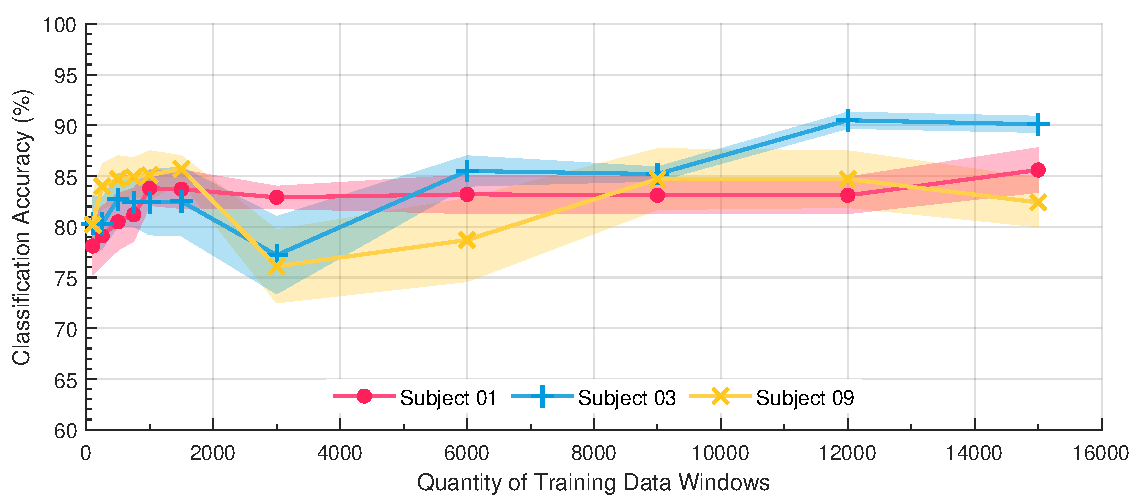
\includegraphics[width=\textwidth]{content/5-Personalisation/ch5_pre_trained_moddel_accuracy.pdf}
    \caption[Retraining a pre-trained LSTM model]{\hl{Retraining a pre-trained LSTM model}}
    \label{fig:ch5_pretrained_model}
\end{figure}

%------------------------------------------------------------
\subsubsection{Transfer Learning/Domain Adaptation}
% Mixed training data
% something akin to k-fold for time varying data (General Data set -> Individual Data set -> General Data set -> Individual Data set)

% Freezing individual layers - Illustration of which layers are frozen
\begin{figure}[htbp]
    \centering
    \includegraphics[width=0.95\textwidth]{example-image-duck}
    \caption[Retraining a pre-trained LSTM model]{Retraining a pre-trained LSTM model - frozen dense layer}
    \label{fig:ch5_freezing_dense_layer}
\end{figure}

\begin{figure}[htbp]
    \centering
    \includegraphics[width=0.95\textwidth]{example-image-duck}
    \caption[Retraining a pre-trained LSTM model]{Retraining a pre-trained LSTM model - frozen LSTM layer}
    \label{fig:ch5_freezing_LSTM_layer}
\end{figure}

% Adding additional layers
\begin{figure}[htbp]
    \centering
    \includegraphics[width=0.95\textwidth]{example-image-duck}
    \caption[Retraining a pre-trained LSTM model]{Retraining a pre-trained LSTM model - train new LSTM layer}
    \label{fig:ch5_additional_LSTM_layer}
\end{figure}

\section{Discussion}

Bias the data set towards the target data, using the general population to supplement the limited environments experienced by the subject. Similar to Balanced Batch Learning \cite{Cruciani2020}
% Have we met the research aims

% Do any of the methods show promise

\section{Conclusions}
% What have we achieved

% What are we going to do next
